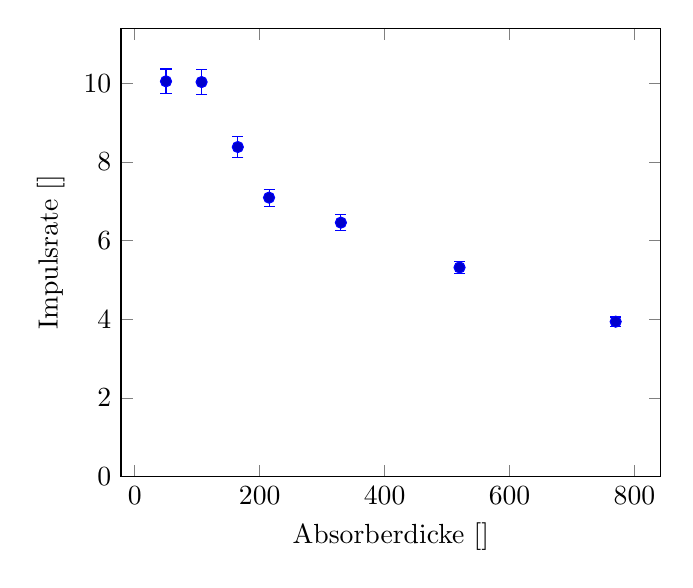
\begin{tikzpicture}
\begin{axis} [
%enlargelimits=.15,
%ybar,
%symbolic x coords={excellent, good, neutral},
%xtick = data,
error bars/y dir = both,
error bars/y explicit,
only marks,
ymin = 0,
%ymode=log,
xlabel={Absorberdicke [\si{\micro\meter}]},
ylabel={Impulsrate [\si{\per\second}]}
]
\addplot table[x = x, y= y, y error = yerror]  {
x	y	yerror
50	10.045045045	0.3141423395
107	10.0267857143	0.3123132646
165	8.3759398496	0.2587336329
215	7.0891719745	0.2172391352
330	6.4540229885	0.1961323762
520	5.3142857143	0.1610792422
770	3.9363957597	0.1187560548
};
\end{axis}
\end{tikzpicture}